\scanpage{4}
\figure{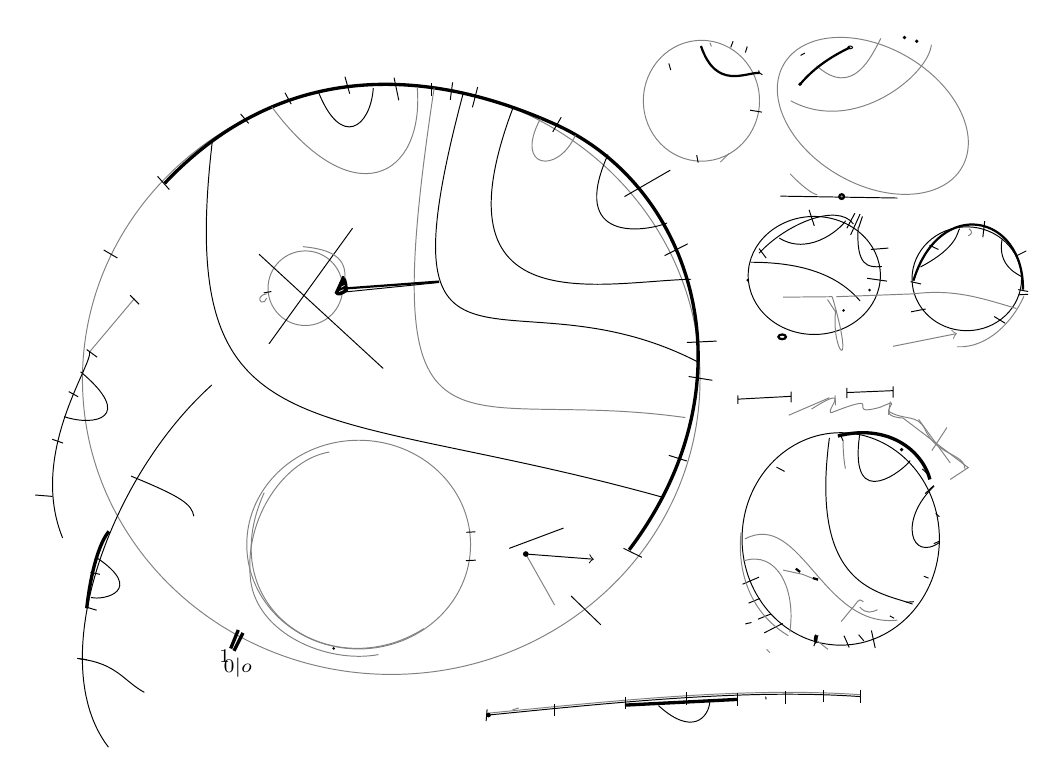
\begin{tikzpicture}[x=.006cm,y=-.006cm,line width=.35pt,every node/.style={font=\scriptsize,inner sep=1pt}]
\draw[gray] (802,865) ellipse(654 and 625);
\draw[very thick] (322,450)..controls(549,209)and(846,186)..(1156,328)..controls(1443,462)and(1574,872)..(1306,1226);
\draw (423,361)..controls(344,1037)and(630,907)..(1374,1114);
\draw[gray] (549,288)..controls(721,520)and(873,438)..(857,246);
\draw (648,257)..controls(696,377)and(758,332)..(764,248);
\draw[gray] (893,247)..controls(763,1108)and(930,876)..(1425,946);
\draw (955,257)..controls(768,960)and(1049,619)..(1453,829);
\draw (1061,287)..controls(885,750)and(1243,658)..(1437,653);
\draw[gray] (1118,313)..controls(1061,419)and(1155,432)..(1192,348); \draw (1261,389)..controls(1177,576)and(1338,553)..(1386,534);
\draw[gray] (163,807)--(258,694);
\foreach \x/\y/\a/\b in {307/435/332/463,193/591/222/608,157/802/179/818,249/687/268/706,483/303/500/323,577/258/590/282,704/224/714/260,808/226/818/274,888/237/888/265,932/236/927/273,985/246/974/289,1162/310/1144/341,1296/478/1393/422,1381/603/1430/578,1428/787/1491/784,1432/859/1482/867,1390/1026/1428/1038,1294/1223/1333/1242,1183/1324/1246/1385}{\draw (\x,\y)--(\a,\b);}
\draw[very thick] (478,1396)--(462,1435) (488,1402)--(469,1440);\node at (477,1475) {$\unsure{0|o}$};\node at (449,1452) {$1$};
\draw[gray] (733,1215) ellipse(237 and 221);\draw[gray] (533,1105)..controls(420,1352)and(677,1516)..(871,1393); \draw[gray] (671,1019)..controls(578,1034)and(489,1157)..(504,1290)..controls(518,1404)and(666,1468)..(775,1448);\draw (961,1189)--(980,1188) (960,1249)--(981,1248);\fill (680,1435) circle(3);
\draw[gray] (620,672) circle(79);\draw (522,600)--(785,842) (543,790)--(720,545);\draw[thick] (698,673)--(903,658);\draw (704,680)--(902,660)--(903,658);\fill (682,682)..controls(687,671)and(696,652)..(698,646)..controls(704,643)and(710,657)..(710,678)..controls(700,687)and(687,692)..(682,682)--cycle;\draw[white,line width=.25pt] (692,679)--(701,675) (696,670)--(703,666);\draw[gray] (615,584)..controls(680,590)and(706,610)..(704,650);\draw (532,682)--(548,679);
\draw[gray] (538,684)..controls(523,686)and(520,697)..(527,701)..controls(532,704)and(536,699)..(538,693);
\draw[gray] (1087,1235)--(1148,1343);\draw[->] (1087,1235)--(1231,1246);\draw (1052,1223)--(1167,1180);\fill (1087,1235) circle(6);
\draw (106,1201)..controls(33,1022)and(171,832)..(163,807);
\draw (144,849)..controls(260,946)and(175,966)..(109,944);\draw (119,891)--(139,902) (84,992)--(107,1000) (48,1110)--(85,1113);
\draw (203,1644)..controls(66,1466)and(201,1076)..(422,877);
\draw[very thick] (157,1350)..controls(166,1270)and(184,1211)..(204,1187);
\draw (177,1242)..controls(282,1312)and(194,1334)..(166,1327);
\draw (251,1070)..controls(358,1114)and(379,1129)..(384,1155);
\draw (142,1457)..controls(221,1467)and(234,1503)..(279,1528);
\draw (137,1456)--(158,1459) (155,1347)--(178,1354) (165,1274)--(185,1278);
\draw[gray] (1459,275) ellipse(123 and 128);\draw[thick] (1458,159)..controls(1490,254)and(1554,214)..(1582,216); \draw[gray] (1477,152)--(1480,160) (1499,405)--(1518,386);\draw (1580,211)--(1582,216)--(1588,220);
\foreach \x/\y/\a/\b in {1390/196/1394/210,1526/149/1521/162,1556/160/1552/173,1562/295/1587/299,1449/390/1452/406}{\draw (\x,\y)--(\a,\b);}
\draw[gray,rotate around={-30:(1822,307)}] (1822,307) ellipse(218 and 145);
\draw[gray] (1703,201)..controls(1781,271)and(1820,178)..(1839,143) (1648,275)..controls(1784,349)and(1941,219)..(1946,156);
\foreach \x/\y in {1668/240,1889/141,1915/149}{\fill (\x,\y) circle(4);}\draw[fill=white,thick] (1756,478) circle(5);
\draw[fill=white] (1774,162) ellipse(5 and 3);\draw (1626,477)--(1874,481); \draw[thick] (1668,240)..controls(1700,202)and(1740,178)..(1774,162);\draw (1669,179)--(1678,174);\draw[gray] (1647,430)..controls(1667,451)and(1692,472)..(1704,474);
\draw (1698,645) ellipse(140 and 125);\draw (1581,598)..controls(1638,536)and(1747,490)..(1781,536);\draw (1624,566)..controls(1693,608)and(1764,535)..(1764,529);\draw (1563,617)..controls(1673,617)and(1748,644)..(1795,699);\draw (1791,543)..controls(1786,625)and(1811,629)..(1841,626);
\foreach \x/\y/\a/\b in {1581/588/1596/608,1687/506/1698/540,1784/513/1767/545,1795/515/1775/559,1800/520/1792/544,1818/590/1855/587,1810/651/1852/657}{\draw (\x,\y)--(\a,\b);}
\draw[fill=white,thick] (1630,775) ellipse(8 and 5);
\fill (1557,655) circle(3) (1760,719) circle(3) (1815,676) circle(3);\draw[gray] (1736,690)..controls(1787,862)and(1734,810)..(1743,722)--(1726,696);
\draw[gray] (1632,691)--(1736,690) (1745,690)--(1908,684);
\draw (2021,652) ellipse(116 and 110);\draw[thick] (1908,656)..controls(1963,476)and(2142,515)..(2140,675);
\draw (1923,627)..controls(2006,583)and(2000,551)..(2006,546) (2096,567)..controls(2084,627)and(2133,644)..(2138,648);
\draw[gray] (2026,546)..controls(2033,552)and(2033,557)..(2024,561);
\draw[gray] (1908,684)..controls(1993,673)and(2053,693)..(2126,715);\draw[gray,->] (1865,795)--(2000,768);\draw[gray] (2000,796)..controls(2066,800)and(2120,740)..(2142,689);
\foreach \x/\y/\a/\b in {1902/658/1924/663,1942/581/1961/590,2059/530/2055/564,2125/604/2147/593,2130/675/2151/679,2130/686/2151/685,1903/722/1934/716,2079/732/2102/746}{\draw (\x,\y)--(\a,\b);}
\draw (1536,907)--(1649,901) (1536,899)--(1536,917) (1649,891)--(1649,914) (1767,893)--(1864,889) (1767,883)--(1767,905) (1865,880)--(1865,904);
\draw[gray] (1692,928)..controls(1792,865)and(1704,951)..(1741,933)..controls(1855,889)and(1755,947)..(1838,924)..controls(1900,896)and(1814,943)..(1886,947)--(2024,1052)--(1986,1077);
\draw (1754,1203) ellipse(209 and 225);\draw[very thick] (1748,985)..controls(1853,958)and(1926,1014)..(1943,1077);
\draw (1730,989)..controls(1687,1309)and(1837,1315)..(1906,1341);
\draw[gray] (1759,995)..controls(1759,1018)and(1761,1040)..(1764,1054);
\draw (1794,983)..controls(1770,1155)and(1893,1052)..(1901,1037);
\draw (1952,1091)..controls(1875,1164)and(1903,1253)..(1964,1210);
\draw[gray] (1551,1203)..controls(1670,1141)and(1715,1393)..(1874,1375) (1547,1250)..controls(1620,1225)and(1660,1312)..(1646,1401);
\foreach \x/\y/\a/\b in {1618/1051/1635/1060,1752/980/1759/995,1927/1055/1942/1069,1546/1299/1581/1284,1559/1339/1583/1329,1579/1373/1606/1362,1592/1402/1631/1382,1706/1407/1697/1430,1761/1408/1772/1433,1792/1406/1803/1419,1819/1397/1827/1434}{\draw (\x,\y)--(\a,\b);}
\draw[gray] (1755,1378)--(1784,1343)..controls(1795,1327)and(1796,1333)..(1802,1336);
\draw[gray] (1794,1347)..controls(1808,1363)and(1821,1358)..(1832,1353);
\fill (1883,1014) circle(4); \draw[gray] (1644,941)--(1730,904) (1742,899)--(1743,920) (1859,912)--(1855,940);
\draw[gray] (1856,933)..controls(1889,953)and(1916,938)..(1932,970)..controls(1956,1026)and(2016,1022)..(2017,1054);
\draw[gray] (1919,950)--(1986,1042) (1979,967)--(1947,1016);
\draw[gray] (1543,1189)..controls(1535,1259)and(1554,1355)..(1643,1408);
\draw[gray] (1632,1269)--(1673,1278)--(1706,1291);\draw[thick] (1659,1266)--(1668,1273) (1695,1286)--(1706,1289);
\draw (1933,1107)--(1951,1090) (1955,1149)--(1963,1156) (1951,1213)--(1963,1208) (1930,1282)--(1940,1286) (1892,1337)--(1909,1336) (1858,1366)--(1867,1371);
\draw[gray] (1706,1420)--(1727,1437) (1597,1437)--(1604,1444);\draw (1552,1383)--(1565,1380);\fill (1701,1415) ellipse(4 and 10);
\draw[gray] (1008,1572)..controls(1282,1545)and(1554,1516)..(1796,1533);\draw (1008,1576)..controls(1282,1549)and(1554,1520)..(1796,1537);\draw[very thick] (1297,1555)--(1534,1543);\fill (1008,1576) circle(5);\draw (1005,1564)--(1003,1589) (1595,1537)--(1596,1543);\draw[gray] (1059,1565)--(1072,1561);
\foreach \x/\y in {1147/1566,1299/1551,1427/1541,1535/1544,1637/1540,1717/1536,1796/1537}{\draw (\x,\y-14)--(\x,\y+13);}\draw (1368,1556)..controls(1440,1622)and(1475,1581)..(1477,1546);
\end{tikzpicture}}

Structure : Graphe segment, avec inv. \inserted{$\sigma$} sur l'ens. des arêtes

\unsure{.} \uline{admissible} se définit par réc sur le nb $n$ d'arêtes (ordre du graphe)
\[
\begin{array}{l|l}
\Gamma\ \text{admissible}&\sigma=\mathrm{id}\\
\text{d'ordre }n\geq1&\text{ou }\exists\ \text{orbite }\inserted{\unsure{\varepsilon|\xi}}\text{ de }\sigma\text{ formée de deux arêtes consécutives,}
\end{array}
\]
\uline{et} le graphe \inserted{$\Gamma'$} déduit de $\Gamma$ par contraction en 1 point de l'une des \deleted{\unsure{deux}} arêtes $\in\unsure{\varepsilon|\xi}$, \deleted{\unsure{est}} muni de l'involution $\sigma'$ déduite de $\sigma$, est admissible

\margin{Tout graphe inv. d'ordre 0 est adm. (ceux d'ordre 1 aussi)}

\figure{\begin{tikzpicture}[x=.006cm,y=-.006cm,line width=.4pt]
\draw (283,2508)..controls(533,2196)and(870,2292)..(1093,2415);
\draw (416,2384)..controls(446,2436)and(451,2474)..(444,2553);
\draw (545,2328)..controls(574,2472)and(706,2460)..(740,2304);
\draw (881,2332)..controls(853,2392)and(851,2460)..(848,2491);
\fill (478,2353) circle(4) (835,2312) circle(4);
\draw[fill=white] (642,2306) ellipse(5 and 3); \fill (1081,2409) circle(2);
\draw[gray] (1373,2540) ellipse(315 and 290);
\draw[gray] (1073,2533)..controls(1008,2771)and(1169,2792)..(1251,2820) (1688,2516)..controls(1704,2737)and(1577,2791)..(1384,2835);
\draw (1248,2813)..controls(1232,2747)and(1368,2735)..(1370,2838);
\draw[gray] (1200,2793)--(1226,2753) (1414,2798)--(1423,2878);
\fill (1203,2788) circle(2.5) (1316,2829) circle(5) (1420,2831) circle(4);\draw[very thick] (1273,2811)--(1272,2821) (1291,2820)--(1290,2830) (1337,2827)--(1339,2838);
\draw (1884,2393) ellipse(93 and 91);
\draw (1792,2434)..controls(1745,2478)and(1713,2491)..(1689,2504) (1858,2308)--(1829,2234) (1924,2307)--(1955,2235) (1952,2451)--(1997,2506);
\draw (1798,2329)--(1813,2341) (1962,2330)--(1951,2340) (1876,2474)--(1873,2494);
\fill (2010,2538) circle(2); \draw[gray] (1061,2574)..controls(1083,2489)and(1109,2482)..(1061,2581);\draw[gray] (1800,2350)..controls(1779,2391)and(1789,2446)..(1841,2460) (1907,2302)..controls(1958,2315)and(1989,2370)..(1976,2433);
\end{tikzpicture}}
\margin{3}
